\section*{Discontinuidades en cuerdas}


\item 
\begin{minipage}[t][1.6cm]{0.6\textwidth}
Nos interesa estudiar la unión de dos cuerdas de distinta densidad lineal $\lambda_{m1}$ y $\lambda_{m2}$, por lo que las consideraremos semi--infinitas. 
Mientras se las somete a una tensión constante, \(T_0\), incide desde la primera una onda $\psi_i(x,t) = A_i \cos{ \left( k_{1} x- \omega t \right) }$.
\end{minipage}
\begin{minipage}[c][-0.2cm][t]{0.34\textwidth}
	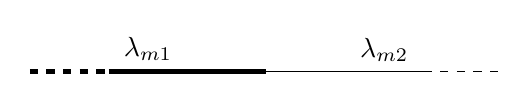
\begin{tikzpicture}[scale= 1]
		\draw [ultra thick, dashed] (-3,0) -- (-2,0);
		\draw [ultra thick] (-2,0) -- (0,0) node [near start, above] {\(\lambda_{m1} \)};
		\draw [thin] (0,0) -- (2,0) node [near end, above] {\(\lambda_{m2} \)}; % node [midway, above] {\(\lambda_{m2} \)};
		\draw [thin, dashed] (2,0) -- (3,0);
	\end{tikzpicture}
\end{minipage}
\begin{enumerate}
	\item Calcule $k_{1}$ y $k_{2}$, es decir, los números de onda a cada lado de la unión.
	\item Plantee la solución más general para $\psi(x,t)$ de cada lado de la unión.
	\item ¿Qué condiciones deben verificarse en el punto de unión de las cuerdas?
	\item Usando b) y c), calcule la perturbación $\psi(x,t)$ en cada una de las cuerdas.
	\item Determine coeficientes de reflexión, $R$, y transmisión, $T$.
	¿Qué sucede en el caso \(\lambda_{m2} \rightarrow \infty\)?
	¿Y sí \(\lambda_{m1} \to \lambda_{m2}\)? 
\end{enumerate}



\item 
\begin{minipage}[t][2.3cm]{0.6\textwidth}
La cuerda de la izquierda, de densidad \(\lambda_{m1}\) y largo \(L\), se encuentra fija en su extremo izquierdo a la pared, y en su extremo derecho a otra cuerda semi-infinita de densidad \(\lambda_{m2}\).
Todo el sistema se encuentra sometido a tensión \(T_0\).
Suponga que por la cuerda de densidad \(\lambda_{m2}\) incide la onda armónica \(\psi_i(x,t) = A_i \mathrm{e}^{i (\omega t + k_2 x) }\).
\end{minipage}
\begin{minipage}[c][0.2cm][t]{0.34\textwidth}
	\begin{tikzpicture}[scale= 1]
		\draw (-2,-1) -- (-2,1); % pared vertical
		\fill [pattern = north east lines] (-2.25,-1) rectangle (-2,1);
		\draw [ultra thick] (-2,0) -- (0,0) node [midway, above] {\(\lambda_{m1} \)};
		\draw [thin] (0,0) -- (3,0) node [midway, above] {\(\lambda_{m2} \)};
		\dimline [extension start length= -0.2, extension end length = -0.2] {(-2,-0.4)}{(0,-0.4)}{\(L\)}; 
		\draw [thin, dashed] (3,0) -- (4,0);
	\end{tikzpicture}
\end{minipage}
\begin{enumerate}
	\item Imponga las condiciones de contorno apropiadas y determine \(\psi(x,t)\) en cada sector de la cuerda.
	\item Halle los valores de \(L\) para los cuales hay un nodo de desplazamiento en la unión de las cuerdas.
\end{enumerate}


\item 
\begin{minipage}[t][1.6cm]{0.6\textwidth}
Una cuerda de densidad lineal \(\lambda_m\) sometida a una tensión \(T_0\) tiene en su centro, \(x= 0\), un pequeño nudo de masa \(M\).
Este causa que sea parcialmente reflejada viajando en la dirección de las \(x\) positivas dada por \(\psi_i(x,t) = A_i \mathrm{e}^{i ( k x - \omega t ) }\).
\end{minipage}
\begin{minipage}[c][-0.5cm][t]{0.34\textwidth}
	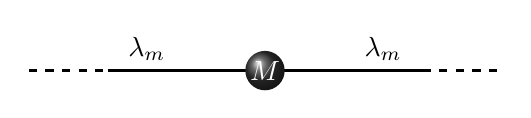
\begin{tikzpicture}[scale= 1]
		\draw [thick, dashed] (-3,0) -- (-2,0);
		\draw [thick] (-2,0) -- (0,0) node [near start, above] {\(\lambda_m \)};
		% \draw [thick] (-2,0) -- (2,0); % node [midway, above] {\(\lambda_{m2} \)};
		\draw [thick] (0,0) -- (2,0) node [near end, above] {\(\lambda_m \)};
		\draw [thick,dashed] (2,0) -- (3,0);
		\shade [ball color=black!80] (0,0) circle(0.25) node [] {\color{white} $M$};
	\end{tikzpicture}
\end{minipage}
\begin{enumerate}
	\item Plantee la solución más general para la onda \(\psi (x,t)\) a cada lado del nudo,
	\item y las condiciones de empalme.
	Demuestre que una condición le permite definir que \(A_i + A_r = A_t\) y que la otra implica que \(A_i - A_r = (1 + i \frac{M \omega^2}{k T} )A_t\).
\end{enumerate}

